\capitulo{7}{Conclusiones y Líneas de trabajo futuras}

En este apartado se va comentar las conclusiones del proyecto, además de una explicación sobre las mejoras que se podrían realizar sobre éste.

\section{Conclusiones}
El proyecto merece la pena porque permite comunicarse con personas gravemente afectadas  que sin este no podrían. Sobre todo en los aspectos más relevantes que son la interpretación de emociones negativas que nos permiten saber cuando le ocurre algo malo al paciente, que por desgracia, no nos lo puede decir por su propia voz.

El proyecto ha sido complicado, personalmente el proyecto más costoso en cuanto a tiempo requerido que he hecho, pero tanto desde el equipo de desarrollo de la Universidad de Burgos como desde APACE Burgos estamos contentos con el desenlace de éste.

En primer lugar, porque hemos cumplido todos los objetivos que nos habíamos propuesto al comienzo del proyecto. Al menos todos los objetivos que se ven mostrados en este documento, es decir, los objetivos que dependían directamente de mi trabajo. 

Como comento en el siguiente apartado en las posibles líneas futuras del trabajo, algo que me hubiera gustado probar es el funcionamiento de la aplicación de interpretación con datos de pacientes reales, pero no dependía de nosotros el poder generar los datos suficientes y tampoco se podía forzar a los pacientes a hacer esos sonidos, principalmente porque las emociones con las que hemos trabajado son negativas, ya que tanto desde de APACE como desde la universidad nos parecían más importantes de interpretar.

En segundo lugar, hemos podido, durante todo el proyecto, contar con un punto muy importante, las opiniones de los usuarios finales, es decir, opiniones de padres y madres, de los cuidadores, de los compañeros... Esta es la opinión que realmente nos interesaba. Tanto en las presentaciones a usuarios de la aplicación de generación de datos, como las presentaciones de la aplicación de interpretación he obtenido muy buenas críticas, sobre todo en los apartados hacia los que enfocamos el proyecto, la simplicidad y la accesibilidad.

\section{Líneas de trabajo futuras}
Como ya he comentado en el apartado anterior, he cumplido casi todos los objetivos que tenía en este proyecto, aun así siempre hay puntos donde se puede mejorar. Algunas de estas mejoras son:
\begin{itemize}
	\item Uso de otro tipo de clase para la grabación en \textit{Android}, aunque \textit{MediaRecorder} no me ha dado malos resultados, siempre es mejor usar un grabación sin pérdidas.
	\item Poder tener más datos con los que poder realmente hacer un estudio de la clasificación real.
	\item Poder incluir otro clasificador que nos permita identificar el paciente a partir del audio si tener que ser seleccionado a mano.
	\item Mejorar el aspecto visual de la aplicación de generación de datos para que tenga una mayor accesibilidad.
	\item Poder realizar un estudio, con los datos suficientes, para saber si se puede generalizar el problema y así no tener que hacer un clasificador por cada paciente.
	\item Poder modificar la aplicación para que se asocie a un paciente y grabe siempre que éste emite algún sonido. 
	\item Poder usar la aplicación con personas con otras discapacidades y/o enfermedades.
	\item Poder realizar una aplicación web para poder añadir y eliminar pacientes.
\end{itemize}

\includepdf[pages={6}]{resumendeprensa14-06-19}
